\chapter{Untersuchung der Messdaten}
Um eine Aussage über die Qualität des Touchscreen treffen zu können, werden mehrere Untersuchungen angestellt.

Bei der ersten Untersuchung wird auf die Mitte des Touchscreen gedrückt und die Position wird für eine gewisse Zeit gehalten.
Die Daten werden anschließen ausgewertet (siehe Abschnitt \cref{ab:genau}).

Um die erste Untersuchung zu erweitern wird nun die Mitte des Touchscreen wiederholt gedrückt.
Hier bei soll die Wiederholbarkeit eines Punktes auf dem Touchscreen untersucht werden.
Die Auswertung ist in Abschnitt \cref{ab:wiederholung} zu finden.

Bei der letzten Untersuchung wird die Linearität des Touchscreen untersucht.
Hierfür gibt der Hersteller eine Garantie, unter der sich die Linearität des Touchscreen befinden soll.
Den Wert der angegeben wird liegt bei \SI{1,5}{\%} (siehe \cref{ds:touch} Seite 3 des Datenblatts).

Um die Nachfolgende Untersuchungen korrekt durchführen zu können muss zu nächst der Reaktionsbereich des Touchscreens ermittelt werden.
Durch seine Bauform hat dies einen Randbereich an dem es nicht zuverlässig Werte ausgibt.
Umkehrschluss, das Programm erkennt nicht das etwas den Touchscreen betätigt.
Im Datenblatt werden Werte für den Bereich genannt in dem es zuverlässig arbeitet.
In X-Richtung hat der Touchscreen einen Arbeitsbereich von \SI{214,5}{mm} und in Y-Richtung eine Bereich von \SI{161,0}{mm}.
Diese Werte wurden durch Messungen ermittelt.

Durch Ausprobieren wurden die maximal und minimal ADC-Werte in die jeweilige Richtung ermittelt.
% \begin{table}[ht!]
%     \caption{maximal und minimal ADC-Werte}
%     \begin{center}
%         \begin{tabular}{ c |c| c }
%                 & x-Richtung & y-Richtung \\ \hline
%          max. ADC-Werte & 961 & 917 \\  \hline
%          min. ADC-Werte& 68 & 108 \\   
%         \end{tabular}
%     \end{center}   
% \end{table}

\begin{table}[h]
    \centering
    \caption[Empirisch ermittelter Wertebereich der ADC]{Empirisch ermittelter Wertebereich der ADC für die äußeren Grenzen des Touchscreens in jeweils horizontaler (x) und vertikaler (y) Richtung.}
    \begin{tabular}{@{}lrr@{}}
        \toprule
            &Min    &Max\\
        \midrule
        x   &68     &961\\
        y   &108    &917\\
        \bottomrule
    \end{tabular}
    \label{tab:ADC min max}
\end{table}

Mit diesen Werten lässt sich Arbeitsbereich (in ADC-Werten) des Touchscreen in jede Richtung bestimmen.
\begin{align}
    ADC_{x,len} &= 961 - 68 = 893
    \label{eq:adcxlen}\\
    ADC_{y,len} &= 917 - 108
    \label{eq:adcylen}
\end{align}
Mit diesen Werten (Gleichung \cref{eq:adcxlen} und Gleichung \cref{eq:adcylen}) können im Anschluss die Werte in das metrische System überführt werden und die Auflösung des Touchscreen bestimmt werden.
In x-Richtung ergibt sich eine Auflösung von \SI{0,240}{\frac{mm}{ADC}} und in y-Richtung \SI{0,199}{\frac{mm}{ADC}}.

Diese unterschiedliche Werte haben den Ursprung, dass die ADC-Werte sich in x-Richtung auf eine größere Distanz verteilen als in y-Richtung.

\section{Genauigkeit bei konstanten Koordinaten}
\label{ab:genau}
Bei dieser Untersuchung wurden zwei separate Messungen durchführen.
Im ersten Durchlauf wurden die Werte mit dem Medianfilter verarbeitet, bevor sie ausgegeben wurden.
Einen Ausschnitt der Messdaten ist in Tabelle \cref{tab:messgenaufilter} (siehe Seite \cref{tab:messgenaufilter}) dem Bericht beigelegt.
Im zweiten Durchlauf wurden die direkten und ungefilterte Werte ausgegeben.
Hierzu ist ebenfalls ein Ausschnitt der Messdaten beigefügt (siehe \cref{tab:messgenauunfilter} Seite \cref{tab:messgenauunfilter}).
In den Abbildungen \cref{fig:filtered} und \cref{fig:unfiltered} sind die Messdaten der x- und y-Komponenten aufgetragen (siehe Seite \cref{fig:filtered}).

Die Auswertung der Messdaten ist in Tabelle \cref{tab:genaufilter} und \cref{tab:genauunfilter} zu finden.
Bei der Auswertung ist zu beachten das es um zwei separate Messreihen handelt.
Daher hat auch die ungefilterte Messreihe eine Standardabweichung und Varianz von Null, im Vergleich zur gefilterten Messreihe.
Im Normalbetrieb ist der Medianfilter im Programm aktiv, daher haben die Werte der gefilterten Messreihe eine höhere Relevanz.
Die Genauigkeit des Touchscreen in beiden Messreihen ist kleiner als die Auflösung, was auf ein akkurat arbeitenden Touchscreen schließen lässt.
\begin{table}[ht!]
    \caption{Auswertung der gefilterten Messdaten }
    \begin{center}
        \begin{tabular}{ |c|c|c|c|c|c|c| }
          \hline&\multicolumn{2}{c|}{Median}& \multicolumn{2}{c|}{Standardabweichung}&\multicolumn{2}{c|}{Varianz} \\ \hline
         Einheit    &(ADC)              &mm             &(ADC)          &mm             &(ADC)      &mm\\\hline
         x-Richtung & \SI{499,0}{}      & \SI{119,861}{}&\SI{0,0}{}     &\SI{0,0}{}     &\SI{0,0}{} & \SI{0,0}{} \\  \hline
         y-Richtung & \SI{509,999}{}    & \SI{101,495}{}&\SI{0,049}{}   &\SI{0,010}{}   &\SI{0,0}{} & \SI{0,0}{} \\ \hline  
        \end{tabular}
        \label{tab:genaufilter}
    \end{center}   
    \caption{Auswertung der ungefilterten Messdaten}
    \begin{center}
        \begin{tabular}{ |c|c|c|c|c|c|c| }
          \hline&\multicolumn{2}{c|}{Median}& \multicolumn{2}{c|}{Standardabweichung}&\multicolumn{2}{c|}{Varianz} \\ \hline
          Einheit &(ADC)&mm&(ADC)&mm&(ADC)&mm\\\hline
          x-Richtung & \SI{499,0}{} & \SI{119,861}{}&\SI{0,0}{}&\SI{0,0}{}&\SI{0,0}{} & \SI{0,0}{} \\  \hline
          y-Richtung & \SI{510,0}{} & \SI{101,496}{}&\SI{0,0}{}&\SI{0,0}{}&\SI{0,0}{} & \SI{0,0}{} \\ \hline  
        \end{tabular}
        \label{tab:genauunfilter}
    \end{center}   
\end{table}


\begin{figure}[ht!]
    \centering
    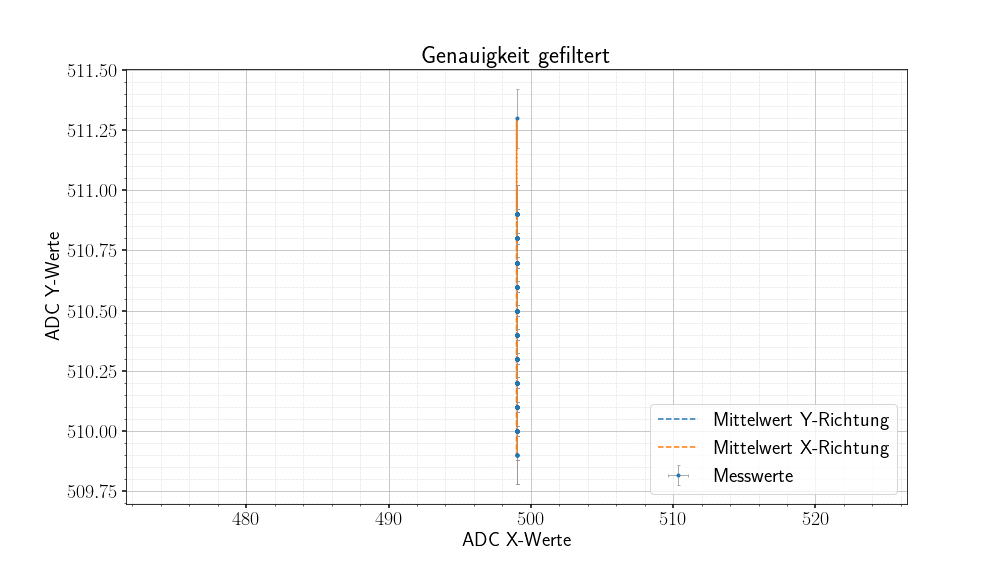
\includegraphics[width=\linewidth]{fig/filtered.png}
    \caption{Darstellung der gefilterten Messreihe}
    \label{fig:filtered}
    \centering
    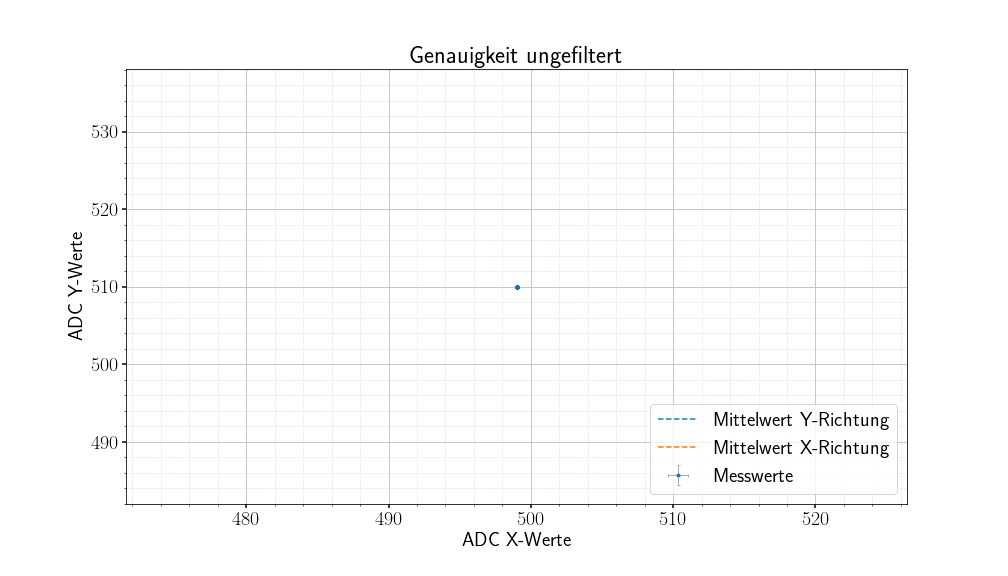
\includegraphics[width=\linewidth]{fig/unfiltered.png}
    \caption{Darstellung der ungefilterten Messreihe}
    \label{fig:unfiltered}
\end{figure}

\newpage

\section{Reproduzierbarkeit von Koordinaten}
\label{ab:wiederholung}
Um die Reproduzierbarkeit von Koordinaten zu untersuchen, wurde die Mitte des Touchscreen mehrmals berührt während die Messdaten aufgezeichnet wurden.
Die Auswertung der Messdaten sind in Tabelle \cref{tab:wiederholung} zu sehen.
Aus den Werten kann man sagen, dass die Genauigkeit der Auflösung entspricht.
\begin{table}[ht!]
    \caption{Auswertung der Reproduzierbarkeit von Koordinaten}
    \begin{center}
        \begin{tabular}{ |c|c|c|c|c|c|c| }
          \hline  
         &\multicolumn{2}{c|}{Median}& \multicolumn{2}{c|}{Standardabweichung}&\multicolumn{2}{c|}{Varianz} \\ \hline
         Einheit    &(ADC)              &mm             &(ADC)          &mm             &(ADC)          &mm\\\hline
         x-Richtung & \SI{510,75}{}    & \SI{122,683}{}&\SI{0,894}{}   &\SI{0,215}{}   &\SI{0,8}{}     & \SI{0,192}{} \\  \hline
         y-Richtung & \SI{515,858}{}    & \SI{102,661}{}&\SI{1,159}{}   &\SI{0,231}{}   &\SI{1,3}{}     & \SI{0,259}{} \\ \hline  
        \end{tabular}
        \label{tab:wiederholung}
    \end{center}   
\end{table}


\begin{figure}[ht!]
    \centering
    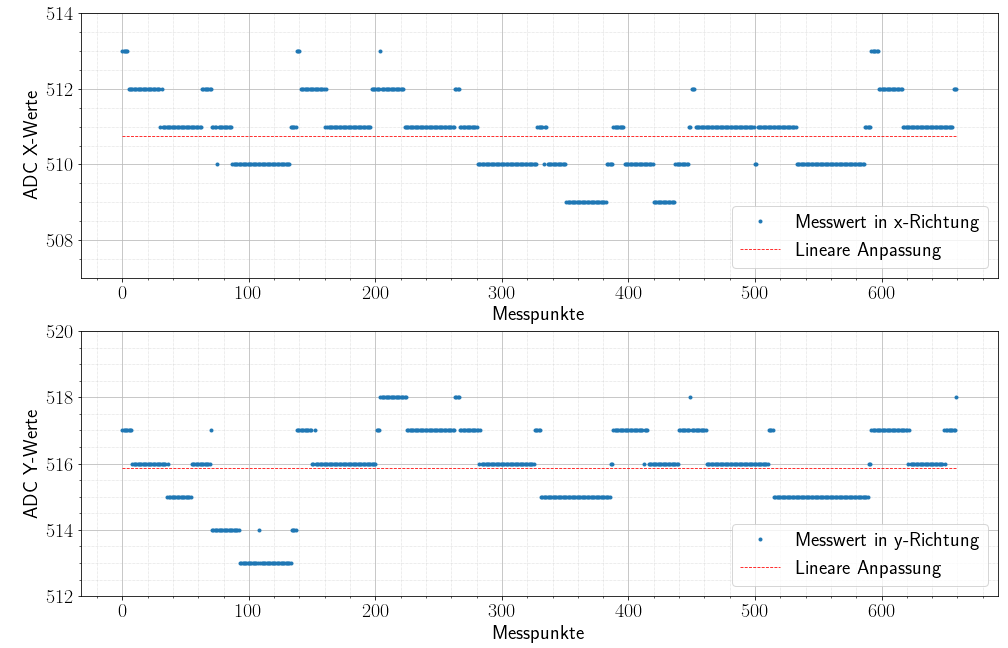
\includegraphics[width=\linewidth]{fig/wiederholung.png}
    \caption{Darstellung der Reproduzierbarkeit von Koordinaten}
    \label{fig:wiederholung}
\end{figure}
\section{Linearität in x- und y-Richtung}
\label{ab:linear}
Um eine Aussage über die Linearität des Touchscreens treffen zu können, wurden in x- und y-Richtung, auf dem Touchscreen alle \SI{10}{mm} eine Markierung gesetzt (siehe \cref{fig:messlinear}).

Die jeweilige Komponenten wurde anschließend jeweils über die physikalische Strecke in einem Diagramm dargestellt (siehe Abb. \cref{fig:xlinear} und Abb. \cref{fig:ylinear}).
Die Messwerte wurden mittels einer linearen Anpassung gefittet (siehe Abb. \cref{fig:xfit} und Abb. \cref{fig:yfit}).

Das \(\chi^2\) gibt Auskunft darüber in welchem Maß Werte miteinander sich verändern.
Je kleiner dieser Wert ist desto eher stimmt die Linearität überein.
Bei der linearen Anpassung in x-Richtung wurde ein \(\chi^2\) von \(0,294\) ermittelt.
Für die Linearität in y-Richtung wurde ein \(\chi^2\) von \(5,946\) ermittelt.

Dadurch das in der Messung bei Abstand 40 mm ein Messpunkt weit von der Messpunktewolke und der dazugehörigen linearen Anpassung abweicht, verzerrt dieser das Ergebnis.

Um Abschließend eine Aussage treffen zu können, ob diese Werte im Wertebereich des Datenblatts sind (Anhang \cref{ds:touch}, Seite \cref{ds:touch}), muss der Grenzwert der Chi-Quadrat-Verteilung mit den Werten der Linearen Anpassung verglichen werden.
Im Datenblatt wird eine Linearität von \SI{1,5}{\%} garantiert.
In der Wertetabelle von \cite{papula} gibt es nur Werte für \SI{1}{\%} oder \SI{2,5}{\%}.
Der gelistete Wert für zwei Freiheitsgrade und für \SI{1}{\%} liegt bei 7,88.
Sowohl das \(\chi^2\) in x-Richtung wie auch in y-Richtung ist kleiner diesem Werte.
Dies hat zur Folge, dass dieser Touchscreen eine Linearität von unter \SI{1}{\%} aufweist.
\begin{figure}
    \begin{minipage}{0.49\linewidth}
        \centering
        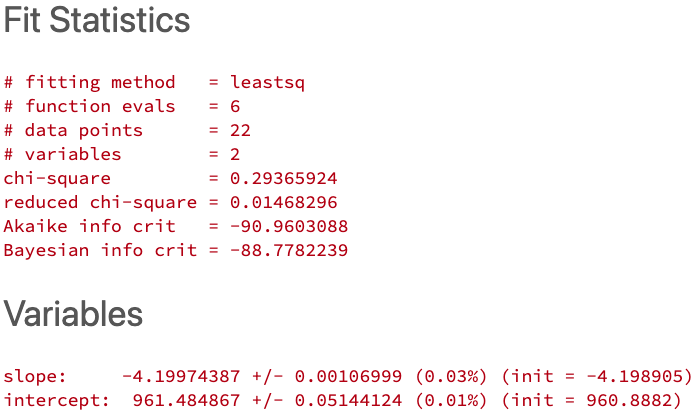
\includegraphics[width=\linewidth]{fig/xfit.png}
        \caption{Auswertung der Linearität in x-Richtung}
        \label{fig:xfit}
    \end{minipage}
    \begin{minipage}{0.49\linewidth}
        \centering
        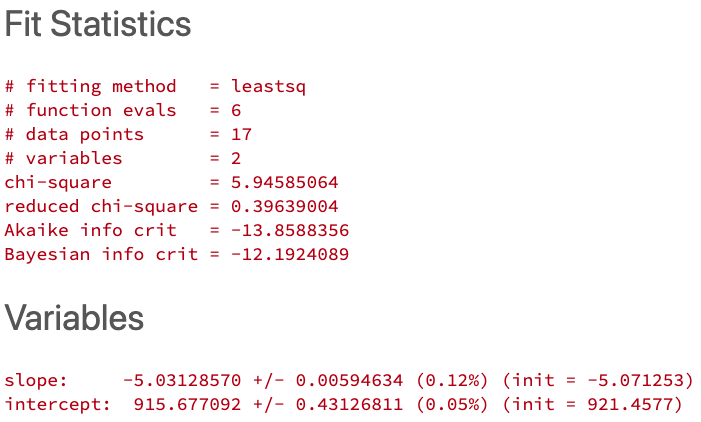
\includegraphics[width=\linewidth]{fig/yfit.png}
        \caption{Auswertung der Linearität in y-Richtung}
        \label{fig:yfit}
    \end{minipage}
\end{figure} 
\begin{figure}[ht!]
    \centering
    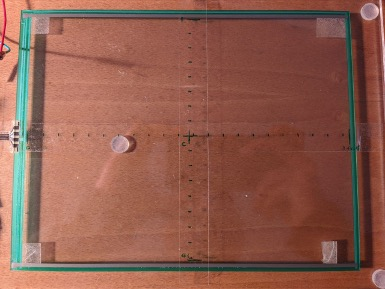
\includegraphics[width=0.6\linewidth]{fig/messlinear.jpg}
    \caption{Messaufbau für Linearität in x- und y-Richtung}
    \label{fig:messlinear}
\end{figure}

\begin{figure}[ht!]
    \centering
    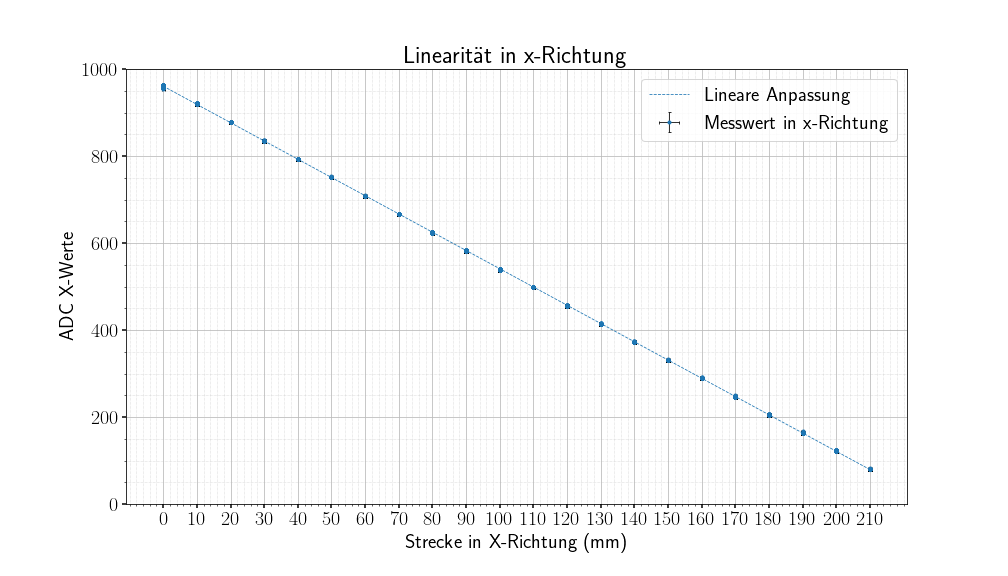
\includegraphics[width=\linewidth]{fig/8_linearitaet_x.png}
    \caption{}
    \label{fig:xlinear}
    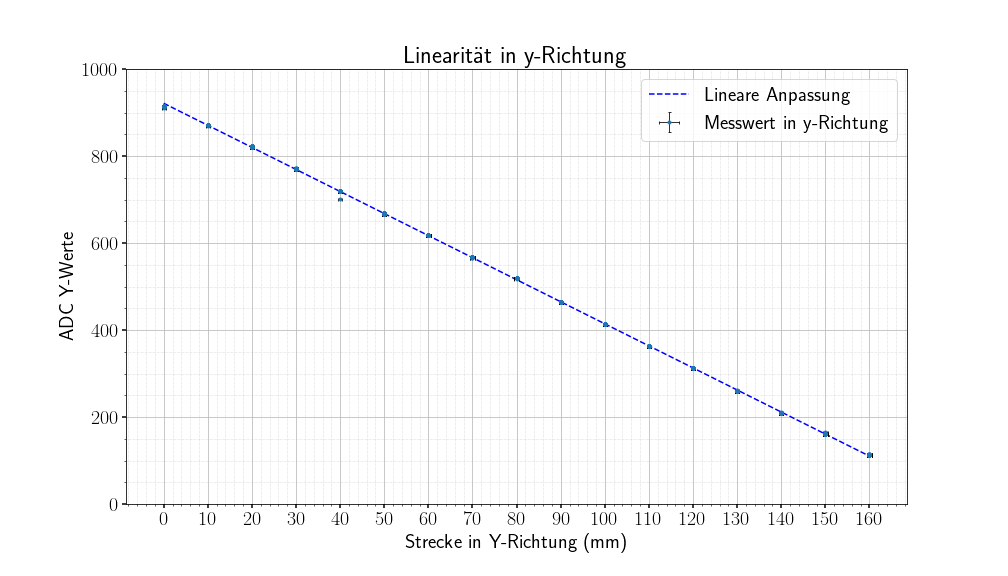
\includegraphics[width=\linewidth]{fig/8_linearitaet_y.png}
    \caption{}
    \label{fig:ylinear}
\end{figure}
